%%%%%%%%%%%%%%%%%%%%%%%%%%%%%%%%%%%%%%%%%%%%%%%%%%%%%%%%%%%%%%%%%%%%%%%%%%%%%
%
% Bayesian prediction of luminosity distribution based on one simulation run:
% An example from TARDIS
%
%%%%%%%%%%%%%%%%%%%%%%%%%%%%%%%%%%%%%%%%%%%%%%%%%%%%%%%%%%%%%%%%%%%%%%%%%%%%%
\documentclass[11pt]{article}
\usepackage[utf8]{inputenc}

\usepackage[a4paper, left=20mm, right=20mm, top=25mm, bottom=25mm]{geometry}
\usepackage[numbers]{natbib}
\usepackage{hyperref}
\usepackage{physics}

\usepackage[colorinlistoftodos]{todonotes} % Use 'disable' to remove todos in final version
\newcommand{\fred}[1]{\todo[color=orange!40,inline]{#1}} %
\newcommand{\fredmargin}[1]{\todo[color=orange!40]{#1}} %
\newcommand{\checked}{\todo[color=green,noline]{\checkmark}} %
\newcommand{\checkedl}{\todo[color=brown]{\checkmark}} %
\newcommand{\hans}[1]{\todo[color=yellow!30,inline]{#1}} %
\newcommand{\hanslong}[2][]{\todo[%bordercolor=red,
  color=white,inline,caption={2do}, #1]{
    \begin{minipage}{\textwidth} #2\end{minipage}}} %

%% CHANGE THIS DATE AS YOU MODIFY THE FILE
\newcommand{\vdate}{161130}
\pagestyle{myheadings}
\markboth{Version \vdate} {Version \vdate}

\parindent=3ex
%%%%%%%%%%%%%%%%%%%%%%%%%%%%%%%%%%%%%%%%%%%%%%%%%%%%%%%%%%%%%%%%%%%%%%%%%%%%%
\usepackage{bm,amssymb,amsfonts,amsmath}  % bold math symbols, AMStex
\usepackage{graphicx}    % standard graphics
%%%%%%%%%%%%%%%%%%%%%%%%%%%%%%%%%%%%%%%%%%%%%%%%%%%%%%%%%%%%%%%%%%%%%%%%%%%%%
\newcommand{\lleq}[1]{\label{#1} }
% TO REMOVE THE LABEL LETTERS FROM THE EQUATION DISPLAY, COMMENT OUT THIS LINE:
\renewcommand{\lleq}[1]{\label{#1} {\scriptstyle {\rm (#1)}} \hspace*{2ex} }

\newcommand{\smA}{{\scriptscriptstyle A}}
\newcommand{\smB}{{\scriptscriptstyle B}}
\newcommand{\smH}{{\scriptscriptstyle H}}
\newcommand{\smK}{{\scriptscriptstyle K}}
\newcommand{\smL}{{\scriptscriptstyle L}}
\newcommand{\smM}{{\scriptscriptstyle M}}
\newcommand{\smN}{{\scriptscriptstyle N}}
\newcommand{\smR}{{\scriptscriptstyle R}}

\newcommand{\smo}{{\scriptscriptstyle 1}}
\newcommand{\smt}{{\scriptscriptstyle 2}}
\newcommand{\smr}{{\scriptscriptstyle 3}}
\newcommand{\smf}{{\scriptscriptstyle 4}}
\newcommand{\smv}{{\scriptscriptstyle 5}}
\newcommand{\smx}{{\scriptscriptstyle 6}}
\newcommand{\sms}{{\scriptscriptstyle 7}}
\newcommand{\sme}{{\scriptscriptstyle 8}}
\newcommand{\smn}{{\scriptscriptstyle 9}}

\newcommand{\bma}{{\bm{a}}}
\newcommand{\bmb}{{\bm{b}}}
\newcommand{\bmc}{{\bm{c}}}
\newcommand{\bmd}{{\bm{d}}}
\newcommand{\bme}{{\bm{e}}}
\newcommand{\bmf}{{\bm{f}}}
\newcommand{\bmg}{{\bm{g}}}
\newcommand{\bmh}{{\bm{h}}}
\newcommand{\bmi}{{\bm{i}}}
\newcommand{\bmj}{{\bm{j}}}
\newcommand{\bmk}{{\bm{k}}}
\newcommand{\bml}{{\bm{\ell}}}
\newcommand{\bmm}{{\bm{m}}}
\newcommand{\bmn}{{\bm{n}}}
\newcommand{\bmo}{{\bm{o}}}
\newcommand{\bmp}{{\bm{p}}}
\newcommand{\bmq}{{\bm{q}}}
\newcommand{\bmr}{{\bm{r}}}
\newcommand{\bms}{{\bm{s}}}
\newcommand{\bmt}{{\bm{t}}}
\newcommand{\bmu}{{\bm{u}}}
\newcommand{\bmv}{{\bm{v}}}
\newcommand{\bmw}{{\bm{w}}}
\newcommand{\bmx}{{{\bm{x}}}}
\newcommand{\bmy}{{\bm{y}}}
\newcommand{\bmz}{{\bm{z}}}
\newcommand{\bmA}{{\bm{A}}}
\newcommand{\bmB}{{\bm{B}}}
\newcommand{\bmC}{{\bm{C}}}
\newcommand{\bmD}{{\bm{D}}}
\newcommand{\bmE}{{\bm{E}}}
\newcommand{\bmF}{{\bm{F}}}
\newcommand{\bmG}{{\bm{G}}}
\newcommand{\bmH}{{\bm{H}}}
\newcommand{\bmI}{{\bm{I}}}
\newcommand{\bmJ}{{\bm{J}}}
\newcommand{\bmK}{{\bm{K}}}
\newcommand{\bmL}{{\bm{L}}}
\newcommand{\bmM}{{\bm{M}}}
\newcommand{\bmN}{{\bm{N}}}
\newcommand{\bmO}{{\bm{O}}}
\newcommand{\bmP}{{\bm{P}}}
\newcommand{\bmQ}{{\bm{Q}}}
\newcommand{\bmR}{{\bm{R}}}
\newcommand{\bmS}{{\bm{S}}}
\newcommand{\bmT}{{\bm{T}}}
\newcommand{\bmU}{{\bm{U}}}
\newcommand{\bmV}{{\bm{V}}}
\newcommand{\bmW}{{\bm{W}}}
\newcommand{\bmX}{{\bm{X}}}
\newcommand{\bmY}{{\bm{Y}}}
\newcommand{\bmZ}{{\bm{Z}}}

\newcommand{\bmalpha}{{\bm{\alpha}}}
\newcommand{\bmbeta}{{\bm{\beta}}}
\newcommand{\bmchi}{{\bm{\chi}}}
\newcommand{\bmdelta}{{\bm{\delta}}}
\newcommand{\bmepsilon}{{\bm{\varepsilon}}}
\newcommand{\bmphi}{{\bm{\phi}}}
\newcommand{\bmgamma}{{\bm{\gamma}}}
\newcommand{\bmeta}{{\bm{\eta}}}
\newcommand{\bmiota}{{\bm{\iota}}}
\newcommand{\bmkappa}{{\bm{\kappa}}}
\newcommand{\bmlambda}{{\bm{\lambda}}}
\newcommand{\bmmu}{{\bm{\mu}}}
\newcommand{\bmnu}{{\bm{\nu}}}
\newcommand{\bmomega}{{\bm{\omega}}}
\newcommand{\bmpi}{{\bm{\pi}}}
\newcommand{\bmpsi}{{\bm{\psi}}}
\newcommand{\bmrho}{{\bm{\rho}}}
\newcommand{\bmsigma}{{\bm{\sigma}}}
\newcommand{\bmtau}{{\bm{\tau}}}
\newcommand{\bmtheta}{{\bm{\theta}}}
\newcommand{\bmupsilon}{{\bm{\upsilon}}}
\newcommand{\bmxi}{{\bm{\xi}}}
\newcommand{\bmzeta}{{\bm{\zeta}}}


\newcommand{\hypo}  {{\mathcal{H}}}  % Model
\newcommand{\ldef}{\;{:}{=}\;}
\newcommand{\rdef}{\;{=}{:}\;}
\newcommand{\realnumbers}{\mathbb{R}}
\newcommand{\integers}{\mathbb{Z}}
\newcommand{\cond}{\,|\,}
\newcommand{\NBD}{\mathrm{NB}}

\newcommand{\refeq}[1]{Eq.~(\ref{#1})}
\newcommand{\reffig}[1]{Fig.~\ref{fig:#1}}
\newcommand{\refsec}[1]{Sec.~\ref{sec:#1}}

\DeclareMathOperator{\Expect}{\mathbb{E}}
\newcommand{\expect}[1]{\Expect\left[#1\right]}
\newcommand{\expectest}[1]{\widehat{\Expect\left[#1\right]}}
\DeclareMathOperator{\GammaDist}{Gamma}
\DeclareMathOperator{\GaussianDist}{\mathcal{N}}
\DeclareMathOperator{\InvGammaDist}{InvGamma}
\newcommand{\Kalpha}{{K_\alpha}}
\newcommand{\Kbeta}{{K_\beta}}
\newcommand{\npack}{{n_p}}
\newcommand{\lmax}{\ell_{\rm max}}
\newcommand{\Lmax}{{L_{\rm max}}}
\newcommand{\Lumtot}{Q}
\newcommand{\lumtot}{q}
\newcommand{\Lum}{L}
\newcommand{\lum}{\ell}
% \newcommand{\rmdx}[1]{\mbox{d} #1 \,} % differential
\newcommand{\rmdx}[1]{\dd{#1}} % differential
\newcommand{\firstDeriv}[1]{\frac{\partial}{\partial #1}}
\newcommand{\secDeriv}[1]{\frac{\partial^2}{\partial #1^2}} % second partial derivative
\newcommand{\secPartial}[2]{\frac{\partial^2}{\partial #1 \, \partial #2}} % second partial derivative
\newcommand{\tardis}{TARDIS}
\DeclareMathOperator{\Variance}{\mathbb{V}}
\newcommand{\variance}[1]{\Variance\left[#1\right]}

%%%%%%%%%%%%%%%%%%%%%%%%%%%%%%%%%%%%%%%%%%%%%%%%%%%%%%%%%%%%%%%%%%%%%%%%%%%%%
\begin{document}

\begin{center}
  \textbf{\Large Bayesian prediction of supernova luminosity  distributions}\\[8pt]
  \textbf{\Large based on simulation output: An example from \tardis}\\[12pt]
\end{center}

\textbf{Abstract} TODO\\

\section{What's left to do}

\subsection{why asymptotic approx. has larger variance}
\begin{enumerate}
  \item For $\alpha=1.5, \beta=60, n=14000$ still get 50 \% larger uncertainty from asymptotic compared to summation over $N$. Is it due very asymmetric one-packet distribution? Try larger $\alpha$, for example $\alpha = 30$.
  \item  Another option: $\int \rmdx{\alpha} \rmdx{\beta}$, use true values in simulation. Where does uncertainty come from? From $\lambda$ or $\mu, \sigma^2$?
  \item Are finite number of terms in $\sum_N$ a problem? Check
\end{enumerate}

\subsection{Plots}

\begin{enumerate}
  \item generate a toy spectrum, take frequencies from actual tardis,
  generate luminosities from a $\GammaDist(\alpha, \beta)$, no $\nu$
  dependence of $\alpha, \beta$ for clarity , plot spectrum with
  uncertainty bands, show it early in the paper, then describe where
  it comes from
  \item compare asymptotic and $\sum_N$ $p(\Lumtot \cond \bmy)$ on a
  plot, add what happens if only $\sqrt{n}$ uncertainty is used: that
  would neglect uncertainty on the single-packet distribution, show
  case when parameters determined from a single bin with few samples,
  should make large difference. Fix $\lambda$, what are the uncertainties now?
  \item Statistics of replicas: again compare \refeq{spe} to \refeq{ral}. Teach a lesson: from a single data set, prediction will be centered there
  \item Question: does Wolfgang want to see a plot in which ``$\lambda$ is divided out''? That is , just plot how mean
\end{enumerate}

\subsection{tardis}

move tardis section into separate document in this git repo. Better to keep it out of the paper. Cite tardis when showing the toy spectrum. Mention that in reality $\alpha$ and $\beta$ are $\nu$ dependent

\section{Introduction (Wolfgang)}

\subsection{Astrophysical context}

\textbf{Define here?}
\begin{enumerate}
\item Basic notation for packets, luminosity as used below
\end{enumerate}

\textbf{Issues that need to be resolved}
\begin{enumerate}
\item Write everything in terms of frequency $\nu$ or wavelength $\lambda$
\end{enumerate}

\subsection*{Main points of this paper}

\begin{enumerate}
\item The first goal of this paper is to show that the Bayesian
  approach to this problem is well-founded and robust.

\item Luminosity data generated by a single simulation provides a
  basis for predicting its uncertainty, i.e.\ how much this luminosity
  can be expected to vary from simulation to simulation.

\item The uncertainty in the luminosity calculated in the Bayesian
  approach is larger than anticipated because it takes into account
  not only the variability of the luminosity per packet, but also the
  distribution of the number of packets.

\item Traditional methods using conventional counting ratio
  (``relative frequency'') can also make predictions for such
  uncertainties, but only if the number of packets is large. By
  contrast, the Bayesian method presented here remains valid also for
  small packet multiplicities.

\end{enumerate}

%%%%%%%%%%%%%%%%%%%%%%%%%%%%%%%%%%%%%%%%%%%%%%%%%%%%%%%%%%%%%%%%%%%%%%%%%%%%%
\subsection{Bayesian prediction}
\label{sec:bayp}

We first sketch the generic notation and relations for Bayesian
probability theory.
%
A particular experiment or simulation generates
\textit{data}
which will often come in the form of a list of $n$ measurements,
$\bmy = (y_1,y_2,\ldots,y_n)$. In order to understand or explain this
data, the observer constructs one or more \textit{models} or
\textit{hypotheses} $\hypo$. Central to this construction is the
specification of a \textit{likelihood} $p(\bmy\cond \bmtheta,\hypo)$
where $\bmtheta = (\theta_1,\theta_2,\ldots,\theta_K)$ is the set of
unknown parameters specified by the model. The likelihood is the
probability assigned by the model $\hypo$ to the data $\bmy$ when the
parameters $\bmtheta$ are fixed and known.
%
If and when the individual measurements $y_i$ are independent, the
joint likelihood is the product
\begin{align}
  \lleq{bta}
  p(\bmy\cond \bmtheta) &= \prod_{i=1}^n p(y_i\cond \bmtheta).
\end{align}
At this level of analysis, the goal is to find which values for these
parameters provide a satisfactory description of the data. In the
Bayesian context, these parameter values are best described in terms
of the probability of the parameters given the data,
$p(\bmtheta\cond \bmy)$. This so-called \textit{posterior} is related
to the likelihood by Bayes' Theorem,
\begin{align}
  \lleq{bth}
  p(\bmtheta\cond \bmy)
  &= \frac{p(\bmy\cond\bmtheta)\;p(\bmtheta)}
    {p(\bmy)}
    %= \frac{p(\bmy\cond\bmtheta)\;p(\bmtheta)}
    %{\int d\bmtheta'\, p(\bmy\cond\bmtheta')\;p(\bmtheta')}
\end{align}
where $p(\bmtheta)$, the so-called \textit{prior}, is the probability
assigned to the values of the parameters before any data was taken
into account and the \textit{evidence}
\begin{align}
  \lleq{bti}
  p(\bmy) &= \int d\bmtheta'\, p(\bmy\cond\bmtheta')\;p(\bmtheta'),
\end{align}
is fully determined by the likelihood and prior.
%
Prediction of any ``future'' data $Y$ is made not by considering the
likelihood $p(Y\cond\bmtheta_{\rm max})$ using single best-fit
parameter values $\bmtheta_{\rm max}$, but by integrating over all
possible values of the $\bmtheta$ in terms of the posterior
$p(\bmtheta\cond n,\bml)$,
\begin{align}
  \lleq{btj}
  p(Y\cond \bmy) &= \int d\bmtheta\,p(Y\cond\bmtheta)\,p(\bmtheta\cond \bmy).
\end{align}
The above relations are true for any type of data and can be applied
to actual experimental data and the pertinent physical parameters. The
scope of this paper, however, is limited to the relationship between
simulated data generated by radiative transfer simulation codes.
Likewise, all parameters considered below relate strictly to model
descriptions of the simulation.

%%%%%%%%%%%%%%%%%%%%%%%%%%%%%%%%%%%%%%%%%%%%%%%%%%%%%%%%%%%%%%%%%%%%%%%%%%%%%
\section{From single-simulation data to many-simulation prediction}

% \subsection{Output data from radiative transfer simulations}
\subsection{Simulation data}

We consider a single computer simulation which generates a luminosity
spectrum from $\npack$ photon packets, each with a particular
frequency $\nu_i$ and luminosity $\lum_i$. Together, these frequencies
and luminosities form the raw simulation data
$\bmy = \{ (\nu_i,\lum_i): i = 1,\ldots,\npack\}$.  We divide up the
frequency spectrum into bins of width $\Delta\nu$ centered on
frequencies $\nu_b$ resulting in bin intervals
$\Delta_b = [\nu_b {-} \tfrac{1}{2} \Delta\nu \,,\, \nu_b {+}
\tfrac{1}{2} \Delta\nu], b = 1,2,\ldots, B$. Let $n_b$ be the number
of packets having a frequency falling into a particular bin $b$, and
let the vector $\bml_b = \{(\ell_{b,j}): j = 1,\ldots,n_b\}$ be the
set of luminosities of those packets. The data set is correspondingly
cast into the more compact histogram form
\begin{align}
  \lleq{sdb}
  \bmy = \{(n_b,\bml_b): b = 1,\ldots,B\}
\end{align}
with loss of information limited to replacing the exact packet
frequencies $\nu_i$ by the appropriate $\nu_b$. The total luminosity
in bin $b$ is the sum of luminosities of those packets whose frequency
falls into $\Delta_b$,
\begin{align}
  \lleq{sdc}
  \lumtot_b
  % &= \sum_{i=1}^\npack \bm{1}_{\Delta_b}(\nu_i)\,\ell_i
  &= \sum_{j=1}^{n_b} \lum_{b,j}.
\end{align}
% where the indicator function $\bm{1}_{[a,b]}(x) = 1$ when $x$ is in
% the interval $[a,b]$ and 0 otherwise.

\subsection{Prediction of luminosity spectrum}

Within a given model $\hypo$, the data $\bmy$ is only one of many
possible realisations of the corresponding random variables; for
example, starting the simulation with a different seed would result in
different output data. We denote the general random variables by the
corresponding upper-case symbols,
\begin{align}
  \bmL_b &= \{(\Lum_{b,j}): j = 1,\ldots,N_b\}\\
  \bmY &= \{(N_b, \bmL_b): b = 1,\ldots,B\},\\
  \Lumtot_b &= \sum_{j=1}^{N_b} \Lum_{b,j},
\end{align}
with corresponding likelihood $p(\bmY\cond\bmtheta)$ and posterior
$p(\bmtheta\cond\bmY)$ for any $\bmY$. The lower-case $(n_b,\bml_b)$
are strictly reserved for the simulated data at hand.


The goal of this paper is to illustrate how the single-simulation data
$\bmy$ can be used to predict the distribution of total bin
luminosities $Q_b, b = 1,\ldots,B$ if many simulations had been
carried out.


Various features such as absorption lines make the luminosity spectrum
highly variable. The model we develop below takes into account this
variability in a two-step process. First, the number of packets $N_b$
is modelled by means of a separate Poisson distribution
$p(N_b\cond\lambda_b)$ for each bin, where the parameter $\lambda_b$
will capture most of the variability of the spectrum.  Second, the
single-packet luminosity distribution is modelled by means of a packet
likelihood for $\Lum_{b,j}$ with packet parameters, a packet prior and,
of course, packet parameter posterior. The packet parameters, which
depend on the frequency bin, will be calculated in two ways: first by
drawing them from a ``parametrisation of the parameters'' across all
bins as shown in \refsec{example} and secondly by assuming that
\refsec{asymptotic}



Our approach
is to predict each bin's luminosity $Q_b$ separately using the same
model but allowing its parameters to vary independently in each bin.
Connections between them


function of frequency. In a binned analysis, we can avoid these
difficulties associated to modeling $n_b$. Our approach, however,
requires an explicit expression of how the distribution of the
luminosity of a single packet in our simulation changes with $\nu$. It
is this crucial piece of information that allows us to extend previous
methods in dealing with the extreme cases when the number of packets
in a bin, $n_b$, is one or even zero.



To keep it simple, we shall assume that all bins are independent,
meaning that
\begin{align}
  p(Q_1,Q_2,\ldots,Q_B\cond\bmy) = \prod_{b=1}^B p(Q_b\cond n_b,\bml_b).
\end{align}
Below, we calculate $p(Q_b\cond n_b,\bml_b)$ for fixed $b$ and hence
drop the subscript, i.e.\ $Q_b\to Q, n_b \to n, N_b\to N$ etc.

%%%%%%%%%%%%%%%%%%%
\fred{Refs: Zech, maybe others, too}

In terms of the generic notation of Section \ref{sec:bayp}, Bayesian
prediction of the distribution of the bin's luminosity
$Q = \sum_{j=1}^n L_j$ given the bin's data $(n,\bml)$ is obtained by
considering not only the likelihood $p(Q\cond\bmtheta_{\rm max})$
using best-fit parameter values $\bmtheta_{\rm max}$, but by
integrating over all possible values of the $\bmtheta$ in terms of the
posterior $p(\bmtheta\cond n,\bml)$,
\begin{align}
  p(Q\cond n,\bml) &= \int d\bmtheta\,p(Q\cond\bmtheta)\,p(\bmtheta\cond n,\bml).
\end{align}
The model's parameters $\bmtheta$ and calculation of this prediction
will be set out in detail below.

\section{Model} \label{sec:model}

We consider the total number of packets $\npack$ fixed, for example
chosen by a user. In contrast, the number of packets in a bin, $n_b$
is a realization of a random variable $N_b$ which we assume to follow
a Poisson distribution. With this assumption, we neglect bin-by-bin
correlations and treat each bin independently. From now on, we focus
on a single bin and drop the subscript $b$. Hence
\begin{align}
  \lleq{caa}
  p(N\cond\lambda) &= \frac{e^{-\lambda}\lambda^N}{N!}
  \qquad N = 0,1,\ldots,\infty ,
\end{align}
where the dependency of the Poisson mean, $\lambda>0$, on the bin, or
respectively the frequency $\nu$, is implicit. Let $\bmL = (\Lum_1,\dotsc,\Lum_N)$ denote the
collection of luminosities of packets in the bin, then the total
luminosity in that bin is
% and its realization based on the data $\bmy$ are
\begin{align}
  \lleq{cab}
  \Lumtot &= \sum_{j=1}^{N} \Lum_j%, \qquad \lumtot = \sum_{j=1}^{n} \lum_j
  \,.
\end{align}
The distribution of the luminosity for each packet,
$p(\Lum \cond \bmphi)$, depends on parameters $\bmphi$ and potentially
on the frequency but we suppress the latter dependency.  The packets
are logically independent. Since $N$ follows a Poisson distribution,
$\Lumtot$ follows a \emph{compound Poisson process}.
%
The key quantity of interest is the distribution of $\Lumtot$ given
the data $\bmy$, $p(\Lumtot \cond \bmy)$ for the compound Poisson
process. In the following, we rewrite $p(\Lumtot \cond \bmy)$ to
obtain an expression that we can readily evaluate numerically. Using
the law of total probability,
\begin{align}
  \lleq{qaa}
  p(\Lumtot \cond \bmy) &= \int \rmdx{\bmphi} p(\bmphi \cond \bmy) p(\Lumtot \cond \bmphi, \bmy) \,,
\end{align}
where the first term in the integral is the posterior $p(\bmphi \cond \bmy)$ after observing $\bmy$. We can decompose the second term as
\begin{align}
  \lleq{qab}
  p(\Lumtot \cond \bmphi, \bmy) &= \sum_{N=0}^\infty  p(N \cond \bmphi, \bmy) p(\Lumtot \cond N, \bmphi, \bmy)\,,
\end{align}
where $p(N \cond \bmphi, \bmy) = p(N \cond \lambda)$ is given by
\refeq{caa} and the second term in the sum is
\begin{align}
  \lleq{qac}
  p(\Lumtot \cond N, \bmphi, \bmy) &= \int \rmdx{\bmL} p(\Lumtot \cond \bmL, N, \bmphi, \bmy) p(\bmL \cond N, \bmphi, \bmy)\\
  \lleq{qaf}
  &= \int \rmdx{\bmL} \delta \left( \Lumtot - \sum_{j=1}^N \Lum_j  \right) \prod_{j=1}^N p(\Lum_j \cond \bmphi)\,,
\end{align}
hence $Q$ does not depend on $\bmy$ explicitly. In the next
subsections, we provide more details on our assumptions and provide
explicit expressions for \refeq{qaa}--\refeq{qaf}.

% As the reference frequency, we choose the bin center.

\subsection{Modeling the packet luminosity} \label{sec:pack-lum}

In general, the distribution $p(\Lum_j \cond \bmphi)$ could be a of a
different functional form in each bin. For simplicity, we assume it is
identical but may depend on parameters $\bmphi$ that need to be
inferred from $\bmy$.  To simplify the treatment, we assume that the
frequency bins are narrow or equivalently that $p(\Lumtot \cond \bmy)$
does not vary within a bin. This implies that every sample $\Lum_j$ in
the bin follows the same distribution.

What is the role of $\bmphi$? It contains all parameters needed to
model the entire spectrum that have to be learned from $\bmy$. To
begin, we include the Poisson means for each bin
\begin{align}
  \lleq{qad} \bmphi = \left( \bmlambda, \bmxi \right) = \left(
    {\lambda_1,\dotsc,\lambda_{n_b}}, \bmxi \right)\,.
\end{align}
\fred{How }
The number and the luminosity of the packets are assumed independent,
so the posterior factorizes as
\begin{align}
  \lleq{qadd}
  p(\bmphi \cond \bmy) = p(\bmlambda \cond \bmy) p(\bmxi \cond \bmy) \,.
\end{align}

Regarding the additional parameters $\bmxi$, we have essentially two
extreme options; both illustrated below in \refsec{example} and
\refsec{asymptotic}. The first option is to assume an explicit
\emph{parametric} form, for example some function $f$, such that
\begin{align}
  \lleq{qae}
  p(\Lum \cond \bmphi) = f(\Lum \cond \bmxi, \nu) \,,
\end{align}
where we now made the dependency on $\nu$ explicit again.  In this
way, we assume the same distribution for all frequencies and we only
need to learn the probable values of $\bmxi$ from the data $\bmy$,
$p(\bmxi \cond \bmy)$. The advantage is that $f(\Lum \cond \bmxi, \nu)$ may
be well constrained by $\bmy$ if $\npack$ is large and it is easy to
include further assumptions; e.g., $f$ should be continuous in $\nu$.

The second option is preferable if it is impossible to elicit an
appropriate explicit expression for $p(\Lum \cond \bmphi)$ \emph{and}
each bin has many packets; i.e., $n \gg 1$. Then we can include one or
more parameters for each bin, consider each bin independently, and
perform a \emph{nonparametric} analysis. Compared to the parametric
approach, we now typically have many more parameters, and each one is
determined only by the packets in one instead of all bins.

\subsection{Poisson analysis}

In order to constrain the Poisson mean $\lambda$ in a bin, we have one
measurement, the number of packets $n$ in that bin. Using Bayes' theorem, we find the posterior
\begin{align}
  \lleq{pmd}
  p(\lambda\cond n) %
  &= \frac{p(n\cond\lambda)\,p(\lambda)} {p(n)}
  \ =\ \frac{p(n\cond\lambda)\,p(\lambda)} %
  {\int \rmdx{\lambda} p(n\cond\lambda)\,p(\lambda)} \,.
\end{align}
% to find the posterior predictive of $N$ given $n$ taking into account
% all possible values of $\lambda$,
% \begin{align}
%   \lleq{pme}
%   p(N\cond n)
%   &= \int \rmdx{\lambda}p(N,\lambda\cond n)
%   \ =\ \int \rmdx{\lambda} p(N\cond\lambda, n)\,p(\lambda\cond n)
%   \ =\ \frac{\int \rmdx{\lambda} p(N\cond\lambda)\,p(n\cond\lambda)\,p(\lambda)}
%   {\int \rmdx{\lambda} p(n\cond\lambda)\,p(\lambda)}
% \end{align}
% where $p(N\cond\lambda,n) = p(N\cond\lambda)$ is independent of $n$.
Common uninformative priors are
\begin{align}
  \lleq{pmf}
  p(\lambda) = c \lambda^{-a},
\end{align}
where $a=0$ gives the uniform prior\footnote{For a uniform prior, the
  case $a{=}0$, we require of course a maximum $\lambda_{\rm max}$. As
  long as $\lambda_{\rm max}$ is large enough, the integral can
  effectively be taken to infinity.}, $a=1/2$ gives the Jeffreys and
reference prior, and $a=1$ is the transformation-group result
advocated by Jaynes~\cite[Ch. 12]{jaynes2003probability}. All choices
lead to an improper prior but the posterior is proper provided that
$n \ge 1$; i.e., at least one packet is observed in the bin. The
standard result for the posterior is
\begin{align}
  \lleq{pms}
  p(\lambda\cond n) &= \GammaDist(\lambda \cond \alpha = n-a+1, \beta = 1)\,,
\end{align}
where the  $\GammaDist$ distribution with shape parameter $\alpha$ and rate
parameter $\beta$ is defined as
\begin{align}
  \lleq{gma}
  \GammaDist(\lambda | \alpha, \beta) = \frac{\beta^\alpha}{\Gamma(\alpha)} x^{\alpha-1} e^{-\beta x}\, , \; x > 0 .
\end{align}
% \begin{align}
%   \lleq{pmg}
%   p(n) &= %
%   \int_0^\infty d\lambda\, p(n\cond\lambda)\,p(\lambda)
%   \ =\
%   c \int_0^\infty d\lambda\, \frac{e^{-\lambda}\,\lambda^{n-a}}{n!}
%   \ =\ c\frac{(n-a)!}{n!} \, ,
%   \\
%   \lleq{pmh}
%   p(N\cond n) %
%   &= \frac{n!}{(n-a)!} \int_0^\infty d\lambda\,
%   \frac{e^{-2\lambda} \lambda^{N+n-a}}{N!\, n!}
%   \ =\ \frac{(N+n-a)!}{N!\,(n-a)!\,2^{N+n+1-a}} \, .
% \end{align}

\section{Example application: \tardis} \label{sec:example}

 The \tardis{} packages simulates supernovae with \fred{Wolfgang's
  favorite description of his package}. Here we focus on the real
packets as opposed to the virtual packets output by tardis.

% Based on staring at the distribution of luminosities,
To apply \refeq{pmp}, we first need to choose $P(\Lum_j \cond \bmphi,
\nu)$. A histogram of the luminosities from a \tardis{} run indicates
a strongly skewed distribution with a single mode that is close to but
not at the sharp end point $\lmax$. There is a long tail for small
$\ell$. These features can be accomodated by a $\GammaDist$
distribution with shape parameter $\alpha$ and rate
parameter $\beta$
\begin{align}
  \lleq{gma}
  \GammaDist(x | \alpha, \beta) = \frac{\beta^\alpha}{\Gamma(\alpha)} x^{\alpha-1} e^{-\beta x}\, , \; x > 0 .
\end{align}
if we transform the data as
\begin{align}
  \lleq{gmf}
  x_i \equiv 1- \frac{\ell_i}{\lmax} > 0
\end{align}
and similarly for $\Lumtot \to X$ because $\ell$ is bounded from above and
$x$ is bounded from below.  We first take the largest luminosity of
all \tardis{} packets across the entire frequency range and increase
it slightly to avoid numerical difficulties at the end point
\begin{align}
  \lleq{gme}
  \lmax \equiv (1+\epsilon) \times \max_i \ell_i,
\end{align}
where $ \epsilon=10^{-6}$.  We assume the total number of samples
across all bins is large, hence the effect of considering $\lmax$ a
constant independent of the data is negligible. We checked that
leaving $\lmax$ as a free parameter in a fit gave equivalent results.

We infer $P(X \cond \nu, \npack, \bmnu, \bmx)$ and only in the end
transform back to a probability density in $\Lumtot$ via
\begin{align}
  \lleq{gmg}
  p(\Lumtot  \cond \nu,  \npack, \bmnu, \bml) = p(X  \cond \nu,  \npack, \bmnu, \bmx) \frac{1}{\lmax} \,.
\end{align}
To simplify the numerics, we also rescale the frequencies by a
constant from $\mathcal{O}(10^{15})$ to $\mathcal{O}(1)$.  A major
numerical simplification arises because of the $\Lumtot \to X$
transformation. Rewriting the master~\refeq{pmp} formally as
\begin{align}
  \lleq{gmh}
  p(\Lumtot  \cond \nu,  \npack, \bmnu, \bml) = \sum_{N} p(N \cond \nu,  n) p(\Lumtot \cond N,
\nu, \npack, \bmnu, \bml),
\end{align}
we see that the right-hand side is a mixture density. In our
application, the distribution of a single-packet luminosity is narrow
in the sense that the standard deviation relative to the mean is at
the percent level. This implies that $p(\Lumtot \cond \nu, \npack,
\bmnu, \bml)$ has one mode from each $N$ and all modes are clearly
separated. The transformation $\Lumtot \to x$ effects a strong overlap
between the distributions $p(X \cond N, \nu, \npack, \bmnu, \bmx)$
with similar $N$, so $p(X \cond \nu, \npack, \bmnu, \bmx)$ can be well
approximated by a unimodal distribution; see \reffig{hedgehog}.

\begin{figure}[ht]
  \centering
  % 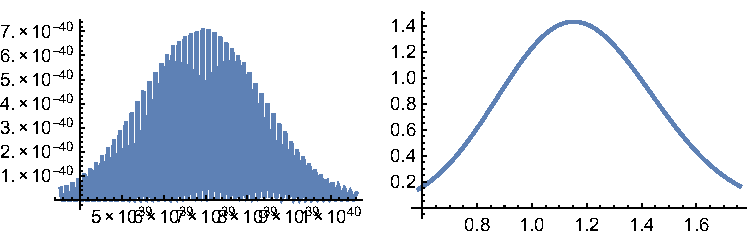
\includegraphics[width=0.48\textwidth]{hedgehog}
  \caption{Left: Prediction $p(\Lumtot \cond  \nu,  \npack, \bmnu, \bml)$, right: $p(x \cond  \nu,  \npack, \bmnu, \bmx)$. I sum over $N$ in both cases. }
  \fred{I still need to pretty this up. I used the old binned approach
    with 50 samples in a bin from which I computed the mean and
    variance to plug into \refeq{gmr} but I computed the sum over $N$
    instead of the integral.}
\label{fig:hedgehog}
\end{figure}

We chose the Gamma distribution because it is \emph{stable}; i.e.,
the sum of $N$ Gamma variates is again a Gamma variate
\begin{align}
  \lleq{gmb}
    X_j \sim \GammaDist(\alpha, \beta) \Rightarrow X \equiv \sum_{j=1}^N X_j \sim \GammaDist(N \alpha, \beta).
\end{align}
Assuming $\alpha = \alpha(\nu \cond \bmphi)$ and $\beta = \beta(\nu
\cond \bmphi)$ are functions of $\nu$ that depend on parameters
$\bmphi$, we set
\begin{align}
  \lleq{gmi}
  p(\bmX \cond \bmphi, N, \nu) &= \prod_{j=1}^N \GammaDist(X_j \cond \alpha, \beta ),\\
  p(\bmx \cond \bmphi, \npack, \bmnu) &= \prod_{i=1}^{\npack} \GammaDist(x_i \cond \alpha_i, \beta_i).
\end{align}
where $\alpha_i \equiv \alpha(\nu_i \cond \bmphi), \beta_i \equiv
\beta(\nu_i \cond \bmphi)$.  Combining \refeq{gmb} and \refeq{gmi}, we
can solve the integral
\begin{align}
  \lleq{gmc}
  \int \rmdx{\bmX} \delta(X - \textstyle\sum_j X_j)
  \,p(\bmX\cond N,\bmphi, \nu) = \GammaDist(X \cond N \alpha, \beta)
\end{align}
implying that the master equation~(\ref{pmp}) considerably simplifies
as
\begin{align}
  \lleq{gmd}
    \boxed{
    p(X\cond \nu, \npack,\bmx,\bmnu)
  = \frac{1}{p(\bmx\cond \npack, \bmnu)}
  \sum_N p(N\cond n)\, \int \rmdx{\bmphi} \GammaDist(X \cond N \alpha, \beta) % p(X \cond N, \bmphi, \nu)
  \, p(\bmx\cond \bmphi, \npack, \bmnu)
  \, p(\bmphi).
  }
\end{align}

\subsection{Linear model}

In the absence of a physical model to determine $\alpha(\nu \cond
\bmphi)$ and $\beta(\nu \cond \bmphi)$, we propose to start with a simple polynomial ansatz   $\alpha(\nu \cond \bmphi) = \sum_{k=0}^\Kalpha \alpha_k \nu^k, \beta(\nu \cond \bmphi) = \sum_{k=0}^\Kbeta \beta_k \nu^k$ such that
\begin{align}
  \lleq{gmp}
  \bmphi = (\alpha_0, \dots \alpha_\Kalpha , \beta_0, \dots \beta_\Kbeta)
\end{align}
The usual trade off between parsimony and the ability to accurately
model the frequency dependence determines the orders of the
polynomials, $\Kalpha$ and $\Kbeta$. This is outside the scope of this
paper. Here we choose $\Kalpha = 3$ and $\Kbeta = 1$.

\subsection{Prior} \label{sec:priors}

The only missing piece to explicitly evaluate \refeq{gmd} is the prior
$p(\bmphi)$. To gain some insight, consider the standard $\GammaDist$
model with $\Kalpha = \Kbeta = 0$.
% There is a conjugate prior but
% unfortunately the normalization constant cannot be evaluated in closed
% form, so it is thus of no use for us.
How about a noninformative prior? The authors of
\cite{moala2013bayesian} present an overview of possible choices and
conclude that the point estimate given by the mode of the posterior is
nearly insensitive to the prior choice starting from around 30
independent identically distributed samples. We posit that there are
this many samples available near any $\nu$ under consideration, so the
form of the prior is not crucial for our application. But there is
some explicit prior information that we want to build into our
analysis. The distribution $p(x \cond \alpha, \beta)$ should always
vanish at the origin. This is equivalent to requiring a maximum away
from the boundary leading to $\alpha > 1$. We choose a uniform prior
on $\bmphi$ on a finite box $V$ through indicator functions
\begin{align}
  p(\bmphi) = \mathbf{1}_{\alpha(\bmphi) > 1}(\bmphi) \mathbf{1}_V(\bmphi).
\end{align}

\subsection{Numerical implementation} \label{sec:numerical}

The box $V$ is chosen by trial and error to be large enough to contain
the relevant region of $p(\bmx\cond \bmphi, \npack, \bmnu)$. For
simple functions $\alpha(\nu \cond \bmphi)$, one can find the minimum
value of $\alpha$ over the entire range of $\nu$ analytically. If this
is too complicated, we propose to require $\alpha(\nu_i \cond \bmphi)
> 1$ only at each packet frequency $\nu_i$. In the evaluation of
$p(\bmx \cond \bmphi, \npack, \bmnu)$, one has to loop over all
packets and compute $\alpha$ and $\beta$ anyways, so the constraint
imposes essentially no computational overhead.  To explicitly evaluate
\refeq{gmd}, we have to overcome the remaining two difficulties: the
integral over $\bmphi$ and the sum over $N$.

As for the former, the posterior $p(\bmphi \cond \npack, \bmnu, \bmx)$
is approximately Gaussian in $\phi$ for $\npack$ large, so we can
apply Laplace's method to perform the $\bmphi$ integrals for both the
evidence $p(\bmx \cond \npack, \bmnu)$ and the posterior mean $p(X
\cond N, \npack, \bmnu, \bmx)$. This requires the Hessian at the mode
and the gradient helps in locating the mode; the analytic expressions
are summarized in \refsec{appendix}.

Regarding the sum over $N$, we start at $N = \lfloor n-a+1 \rfloor =
\arg \max_N p(N|n)$ \fred{Actually we should say $p(N \cond n, a)$}
and continue to larger and smaller values of $N$ until the
contribution to $P(X \cond \nu, \npack, \bmnu, \bmx)$ becomes
negligible. In case the relevant contribution is from large $N$ and
$n$, we interpret $N$ as a continuous variable, replace factorials by
$\Gamma$ function in \refeq{pmh}, and apply Laplace's method to
integrate over $N$ and $\bmphi$.

\fred{Our implementation is available online on \href{https://github.com/tardis-sn/XXX}{github}}

\subsection{Graphical output}

\section{Asymptotic approximation} \label{sec:asymptotic}

In the case that there are many packets in every bin, some
simplifications arise as the exact distribution of individual packets
$p(\Lum \cond \bmphi, \nu)$ becomes irrelevant in the asymptotic
regime $n \to \infty$, which implies $\lambda \to \infty$. In that
case, the compound Poisson distribution can be approximated by a
Gaussian distribution provided that the second moment of
$\Lum, \expect{\Lum^2}$ is finite. To see this in more detail, we define
\begin{align}
  \lleq{ram}
  \mu \equiv \expect{\Lum}, \qquad \sigma^2 \equiv \variance{\Lum}\,.
\end{align}
For a compound Poisson process with arbitrary Poisson mean $\lambda > 0$,
\begin{align}
  \lleq{raa}
  \expect{Q} =\lambda \expect{L} = \lambda \mu, \qquad \variance{Q} = \lambda \expect{L^2} = \lambda (\mu^2 + \sigma^2) \,.
\end{align}

From Theorem 4.3.1 of \cite{bening2002generalized}, we can conclude
that the asymptotic distribution of $\Lumtot$ when
$\lambda \to \infty$, given the first and second moment of $\Lum$, is
\begin{align}
  \lleq{rab}
  P(\Lumtot \cond \bmphi) = \GaussianDist \left( \Lumtot \cond \expect{Q}, \variance{Q} \right) = \GaussianDist \left( \Lumtot \cond \lambda \mu, \lambda (\mu^2 + \sigma^2) \right).
\end{align}
This result is a drastic simplification as it eliminates both the sum over $N$ in \refeq{qab} and the integral over $\bmL$ in \refeq{qaf}.
That allows us to model $\Lumtot$ in each bin \emph{without} making concrete
assumptions about the functional form of $P(\Lum \cond \bmphi)$; i.e., we may now view $\bmphi$ as the collection of first and second moments in each bin in addition to $\lambda$. Continuing the notation of \refeq{qadd},
\begin{align}
  \lleq{rac}
  \bmphi =  \left(\lambda_b, \mu_b, \sigma^2_b \right)_{b=1}^B.
\end{align}
The price for this flexibility is that $\bmphi$ may now contain many
parameters, and each one is determined only from the samples in a
single bin. The joint posterior is
\begin{align}
  \lleq{rad}
  p(\bmphi \cond \bmy ) = \prod_{b=1}^B p\left(\lambda_b, \mu_b, \sigma^2_b \cond \bmy\right),
\end{align}
Focussing on a single bin, we omit the subscript $b$. As before, we
further assume that
\begin{align}
  \lleq{rao}
p(\lambda, \mu, \sigma^2 \cond \bmy) = p(\lambda \cond \bmy) p(\mu,
\sigma \cond \bmy).
\end{align}
The posterior for $\lambda$ is given by \refeq{pms}.  To learn mean
and variance of $\Lum$ from $\bmy$, we follow
Jaynes~\cite[Ch. 7.10]{jaynes2003probability} and assign a Gaussian
sampling distribution
\begin{align}
  \lleq{rae}
  p(\Lum \cond \mu, \sigma^2 ) &= \GaussianDist(\Lum \cond \mu, \sigma^2)
\end{align}
although the actual frequencies may be quite different from a
Gaussian. Our motivation is that this Gaussian represents our state of
knowledge \emph{before} observing $\bmy$ well. To make the
calculations easier, we assume a conjugate prior for unknown $\mu$ and
$\sigma^2$. The standard result for the posterior is
\begin{align}
  \lleq{raf}
  p(\mu, \sigma^2 \cond \bmy) &= \GaussianDist(\mu \cond \mu_0^\prime, \frac{\sigma^2}{n_0^\prime}) \InvGammaDist\left( \sigma^2 \cond \frac{\nu_0^\prime}{2}, \frac{\nu_0^\prime \sigma_0^{\prime 2}}{2} \right)
\end{align}
where the hyperparameters are updated from prior to posterior based on $\bmy$ as
\begin{align}
  \lleq{rag}
  \expectest{\lum} &= \frac{1}{n} \sum_{i=1}^n \lum_i,\\
  \lleq{rah}  n_0^\prime &= n_0 + n,\\
  \lleq{rai}    \mu_0^\prime &= \frac{n_0 \mu_0 + n \expectest{\lum}}{n^\prime},\\
  \lleq{raj}    \nu_0^\prime &= \nu_0 + n,\\
  \lleq{rak}    \nu_0^\prime \sigma_0^{\prime 2} &= \nu_0 \sigma_0^{ 2} + \sum_{i=1}^n \left(\lum_j - \expectest{\lum}\right)^2 + \frac{n_0 n}{n^\prime} \left(\mu_0 - \expectest{\lum}\right)\,.
  \end{align}
  By default, we take a noninformative prior and set
  $n_0 = \mu_0 = \nu_0 = 0$, so the value $\sigma_0^2>0$ is
  irrelevant.
  % The posterior
  % $ p(\expect{\Lum}, \expect{\Lum^2} \cond \bmy)$ is given by
  % \refeq{raf} with $\mu, \sigma^2$ replaced by
  % $\expect{\Lum}, \expect{\Lum^2}$ as indicated in \refeq{rae} because
  % the Jacobian determinant is one.

  Finally all ingredients for the prediction of $\Lumtot$ in one bin are
  ready, and \refeq{qaa} simplifies to
\begin{align}
  \lleq{ral}
  p(\Lumtot \cond \bmy) &= \int \rmdx{\lambda} \rmdx{\mu} \rmdx{\sigma^2} \GaussianDist \left( \Lumtot \cond \lambda \mu, \lambda \sigma^2 \right) p(\lambda \cond \bmy) p( \mu, \sigma^2 \cond \bmy) \,,
\end{align}
where $ p(\lambda \cond \bmy)$ is given by \refeq{pms} and
$ p( \mu, \sigma^2 \cond \bmy)$ by
\refeq{raf}--\refeq{rak}.

\subsection{Numerical implementation}\label{sec:asympt-numeric}

Unfortunately we could not integrate \refeq{ral} analytically but
since the integrand is unimodal and strongly peaked the Laplace or
saddle-point approximation~\cite[Ch. 27]{mackay2003information} can be
applied in two ways. First, if only the value
$p(\Lumtot=\lumtot \cond \bmy)$ for some particular $q$ is sought,
then one can approximate it directly. Second, we can compute the
moments of $\Lumtot$ through the \emph{moment-generating
  function}\fredmargin{ref}
\begin{align}
  \lleq{rap}
  M(t \cond \bmy) = \int_0^{\infty} \rmdx{\Lumtot} p(\Lumtot \cond \bmy) e^{-t \Lumtot} \,
\end{align}
from which the moments are accessible by differentiation
\begin{align}
  \lleq{raq}
  \expect{\Lumtot^k} = (-1)^k \eval{\dv[k]{M(t \cond \bmy)}{t}}_{t=0}
\end{align}

Assuming all involved integrals are absolutely convergent, we can
exchange the order of integration and find
\begin{align}
  \lleq{rar}
  M(t \cond \bmy) &= \int \rmdx{\lambda} \rmdx{\mu} \rmdx{\sigma^2} p(\lambda \cond \bmy) p( \mu, \sigma^2 \cond \bmy)  f(t \cond \lambda, \mu, \sigma^2),
  \intertext{where }
  f\left(t \cond  \lambda, \mu, \sigma^2\right) &\equiv \int \rmdx{\Lumtot} \GaussianDist \left( \Lumtot \cond \lambda \mu, \lambda \sigma^2 \right) e^{-t \Lumtot}= \frac{1}{2} e^{t \lambda (t \sigma^2/2 - \mu)} \left[ 1 + \erf\qty( \frac{\sqrt{\lambda}(\mu - t \sigma^2)}{\sqrt{2 \sigma^2}}) \right].
\end{align}
This implies that the mean and variance of $\Lumtot$ require an integral over the three parameters
\begin{align}
  \lleq{ras}
  \expect{\Lumtot} &= \int \rmdx{\lambda} \rmdx{\mu} \rmdx{\sigma^2} p(\lambda \cond \bmy) p( \mu, \sigma^2 \cond \bmy) \qty(-\eval{\dv{f(t \cond  \lambda, \mu, \sigma^2)}{t}}_{t=0})\\
  \variance{\Lumtot} &= \int \rmdx{\lambda} \rmdx{\mu} \rmdx{\sigma^2} p(\lambda \cond \bmy) p( \mu, \sigma^2 \cond \bmy) \qty(\eval{\dv[2]{f(t \cond  \lambda, \mu, \sigma^2)}{t}}_{t=0}) - \expect{\Lumtot}^2
\end{align}
We implemented the above formulae in the julia language~\cite{julia14}
and used Newton's method from the \texttt{Optim.jl} package in
combination with automatic
differentiation~\cite{RevelsLubinPapamarkou2016} to optimize the
respective integrand and compute the Hessian at the mode. As initial
values, we slightly offset the sample estimates to avoid issues if the
optimizer cannot improve on the initial guess and found convergence
within $\order{10}$ steps:
\begin{align}
  \lleq{rat}
  \qty(\lambda, \mu, \sigma^2) = 1.0005 (n, \expectest{\lum}, \widehat{\variance{\lum}}).
\end{align}
\fred{Did we define expectation value and variance? Should be in notation or intro section}
\fred{At least for us, I should do a comparison plot to evaluate $p(\Lumtot \cond \bmy)$ with both methods }
\fred{We need a plot, the one to compare predictions and 250 real replicas or 100 virtual replicas?}
\fred{Advantage of this approach: no need to store all packets anymore, sum and sum of squares can be accumulated online $\Rightarrow$ reduced computation and storage requirements}

\section{Conclusion} \label{sec:conclusion}

\section{Appendix} \label{sec:appendix}

We use the shorthand $\alpha_n \equiv \alpha(\nu_n \cond
\bmphi), \beta_n \equiv \beta(\nu_n \cond \bmphi), \alpha \equiv
\alpha(\nu \cond \bmphi), \beta \equiv \beta(\nu \cond \bmphi)$.

\subsection{Gradients} \label{sec:gradients}

\begin{align}
  \label{eq:grad-posterior}
  \left( \firstDeriv{\alpha_i}, \firstDeriv{\beta_i} \right) \log p(\bmx \cond \alpha, \beta) &=
  \left(
    \sum_n \left[ \log \beta_n - \Psi(\alpha_n) + \log x_n \right] \nu_n^i \;,
    \sum_n \left[ \frac{\alpha_n}{\beta_n} - x_n \right]\nu_n^i
  \right)
\end{align}

\begin{align}
  \label{eq:grad-prediction}
  \left( \firstDeriv{\alpha_i}, \firstDeriv{\beta_i}, \firstDeriv{N} \right) \log p(X \cond N \alpha, \beta)  &=
  \left(
    \left[ \log \beta - \Psi(N \alpha) + \log X \right] N \nu^i,
    \left[ \frac{N\alpha}{\beta} - X \right]\nu^i,
    \left[ \log \beta -\Psi(N \alpha) + \log X \right] \alpha
  \right)
\end{align}

\begin{align}
  \label{eq:grad-nb}
  \firstDeriv{N} \log p(N \cond n) = \Psi(N+n-a+1) - \Psi(N+1) - \log 2
\end{align}

\subsection{Hessians} \label{sec:hessians}

\begin{align}
  \label{eq:hess-posterior}
    - \left(
    \begin{array}{ccc}
      \secPartial{\alpha_i}{\alpha_j} & \secPartial{\alpha_i}{\beta_j}\\
      \dots & \secPartial{\beta_i}{\beta_j}
    \end{array}
  \right) \log p(\bmx \cond \alpha, \beta)
    &= \left(
    \begin{array}{cc}
      \sum_n \Psi'(\alpha_n) \nu_n^{i+j} & -\sum_n \frac{\nu_n^{i+j}}{\beta_n}\\
      \dots & \sum_n \frac{\alpha_n}{\beta_n^2} \nu_n^{i+j}
    \end{array}
  \right)
\end{align}

 \begin{align}
  \label{eq:hess-prediction}
  & - \left(
    \begin{array}{ccc}
      \secPartial{\alpha_i}{\alpha_j} & \secPartial{\alpha_i}{\beta_j} & \secPartial{\alpha_i}{N}\\
      \dots & \secPartial{\beta_i}{\beta_j} & \secPartial{\beta_i}{N}\\
      \dots & \dots & \secDeriv{N}
    \end{array}
  \right) \log p(X \cond N \alpha, \beta)
  \\
  &=
  \left(
    \begin{array}{ccc}
      N^2 \Psi'(N \alpha) \nu^{i+j} & -\frac{N \nu^{i+j}}{\beta} & \left[ -\log \beta +\Psi(N \alpha) + N \alpha \Psi'(N \alpha) - \log X \right] \nu^{i}\\
      \dots &  \frac{N\alpha}{\beta^2} \nu^{i+j} & -\frac{\alpha}{\beta} \nu^{i} \\
      \dots & \dots & \alpha^2 \Psi'(N \alpha)
    \end{array}
  \right)
\end{align}
\begin{align}
  \label{eq:hess-nb}
   - \secDeriv{N} \log p(N \cond n) = \Psi'(N+1) - \Psi'(N+n-a+1)
\end{align}

\bibliographystyle{plain}
\bibliography{references}


\end{document}
\subsection{Old}
%old text
The joint distribution then is
\begin{align}
  \lleq{cac}
  % Q, N \sim P(Q, N \cond \bmphi, )
  (N,\bmL) &\ \sim\ p(N,\bmL\cond \bmphi,\lambda, \nu)
  = p(\bmL\cond N,\bmphi, \nu)\; p(N\cond \lambda) = \prod_{j=1}^N p(\Lum_j\cond \bmphi, \nu) \; p(N\cond \lambda),
\end{align}
\fred{Do we need this equation?}
where we used that the Poisson term does not depend on $\nu$
explicitly. In general, the distribution of $\Lum_j$ could be a of a
different functional form in each bin. For simplicity, we assume it is
identical but may depend on parameters that differ from bin to bin. In
practice, the distribution of packets usually does not change abruptly
with frequency. We therefore assume that any parameter needed to fully
specify $p(\Lum_j)$ is given explicitly as a continuous function of $\nu$
and the unknown parameters $\bmphi$. This allows us to use a small
number of parameters to describe $p(\Lumtot)$ across the entire frequency
range instead of having a few parameters per bin which could lead to
tens of thousands of parameters for the applications we have in
mind. So we determine $\bmphi$ from fitting all simulated packets
simultaneously whereas $\lambda$ is a per-bin quantity.
\fred{Reformulate when asymptotic approx. included: it has thousands of parameters}

Our goal of predicting $\Lumtot$ in some bin given the simulation output
$(\npack,\bmnu, \bml)$ is captured in the probability density
$p(\Lumtot\cond \nu, \npack,\bmnu, \bml)$ with all relevant parameters
integrated out. To simplify the treatment, we assume that the
frequency bins are narrow or equivalently that $p(\Lumtot \cond \nu, \npack,
\bmnu, \bml)$ does not vary within a bin. This implies that every
sample $\Lum_j$ in the bin follows the same distribution.  As the
reference frequency, we choose the bin center.

% From \refeq{caa}, $N$ does not depend on $\bml$ at all and only
% indirectly depends on $\bmnu$ through $n$.
Since $\Lumtot$ is fully determined by $(N,\bmL)$, it does not depend on
$(\npack,\bml,\bmnu)$, i.e.
\begin{align}
  \lleq{pmi}
  p(\Lumtot\cond N,\bmL,\nu,\npack,\bmnu, \bml)
  = p(\Lumtot\cond N, \bmL)
  &= \delta(\Lumtot - \textstyle\sum_{j=1}^N \Lum_j),
\end{align}
\fred{Uniform order: $\nu$ first, then $\ell$, compare to $S$} where
each $\Lum_j$ is assumed to occur at $\nu$.  Using the law of total
probability repeatedly, we can write the desired distribution as
\fred{Discuss $N=0$ case somewhere}
\begin{align}
  \lleq{pmj}
  p(\Lumtot\cond \nu, \npack,\bmnu, \bml)
  &= \sum_N p(N\cond \nu, \npack,\bmnu, \bml) \, p(\Lumtot\cond N,\nu, \npack,\bmnu, \bml) \\
  \lleq{pmjb}
  &= \sum_N p(N\cond n)\,\int \rmdx{\bmL} p(\Lumtot\cond N,\bmL,\nu, \npack,\bmnu, \bml)\, p(\bmL\cond N,\nu, \npack,\bmnu, \bml)
  \\
  \lleq{pmjc}
  &= \sum_N p(N\cond n)\,\int \rmdx{\bmL} \delta(\Lumtot - \textstyle\sum_{j=1}^N \Lum_j)
  \, p(\bmL\cond N,\nu, \npack,\bmnu, \bml).
\end{align}
The dependence on the simulation output $(\npack,\bmnu, \bml)$ enters
through $p(\bmL\cond N,\npack,\bmnu, \bml)$ in terms of the parameters
$\bmphi$ of $p(\bmL\cond N,\bmphi)$,
\begin{align}
  p(\bmL\cond N,\nu, \npack,\bmnu, \bml)
  &= \int \rmdx{\bmphi} p(\bmL\cond \bmphi,N, \nu, \npack,\bmnu, \bml)\,p(\bmphi\cond N,\nu, \npack,\bmnu, \bml) \\
  \lleq{pmk}
  &= \int \rmdx{\bmphi} p(\bmL\cond \bmphi, N, \nu)\,p(\bmphi\cond N,\nu, \npack,\bmnu, \bml).
\end{align}
because $\bmL$ is fully determined by $N,\bmphi, \nu$ and hence
independent of $\npack,\bmnu, \bml$.  With Bayes' theorem we learn about
$\bmphi$ from the simulation output
\begin{align}
  \lleq{pmkb}
  p(\bmphi\cond N,\nu, \npack,\bmnu, \bml) &=
  \frac{p(\bml\cond \bmphi, N,\nu, \npack,\bmnu)\,p(\bmphi\cond N,\nu, \npack,\bmnu)} %
  {\int \rmdx{\bmphi} p(\bml\cond \bmphi,N,\nu, \npack,\bmnu)\,p(\bmphi\cond N,\nu, \npack,\bmnu)}.
\end{align}
By using a multiplicity- and frequency-independent prior for $\bmphi$,
\begin{align}
  \lleq{pml}
  p(\bmphi\cond N,\nu, \npack,\bmnu) &= p(\bmphi),
\end{align}
and by recognizing that $\bml$ is independent of $N$ and $\nu$
\begin{align}
  \lleq{pmla}
  p(\bml\cond \bmphi,N,\nu, \npack,\bmnu) = p(\bml\cond \bmphi,\npack,\bmnu)
\end{align}
we can write \refeq{pmk} as
\begin{align}
  \lleq{pmn}
  p(\bmL\cond N,\nu, \npack,\bmnu, \bml)
  &= \int \rmdx{\bmphi} p(\bmL\cond N,\bmphi)\, %
  \frac{p(\bml\cond \bmphi, \npack, \bmnu)\,p(\bmphi)} %
  {\int \rmdx{\bmphi} p(\bml\cond \bmphi,\npack,\bmnu)\,p(\bmphi)} \\
  \lleq{pmo}
  &= \frac{1}  {p(\bml\cond \npack, \bmnu)} %
  \int \rmdx{\bmphi} p(\bmL\cond \bmphi, N)\, %
  p(\bml\cond \bmphi, \npack,\bmnu)\,p(\bmphi)
\end{align}
where $p(\bml\cond \npack, \bmnu) = \int \rmdx{\bmphi} p(\bml\cond
\bmphi, \npack,\bmnu)\,p(\bmphi)$ is the evidence.  Inserting \refeq{pmo}
into \refeq{pmjc}, we obtain the desired master equation:
\begin{equation}
  \lleq{pmp}
  \boxed{
  p(\Lumtot\cond \nu, \npack,\bmnu, \bml)
  = \frac{1}{p(\bml\cond \npack, \bmnu)}
  \sum_N p(N\cond n)\,\int \rmdx{\bmL} \delta(\Lumtot - \textstyle\sum_j \Lum_j)
  \displaystyle\int \rmdx{\bmphi} p(\bmL\cond \bmphi, N, \nu) \, p(\bml\cond \bmphi,\npack,\bmnu)
  \, p(\bmphi)
  }
\end{equation}
with
\begin{align}
  \lleq{pmq}
  p(\bmL\cond \bmphi, N, \nu) &= \prod_{j=1}^N p(\Lum_j\cond \bmphi, \nu), \\
  \lleq{pmr}
  p(\bml\cond \bmphi,\npack,\bmnu) &= \prod_{i=1}^{\npack} p(\ell_i\cond \bmphi, \nu_i)
\end{align}
and $p(\cdot \cond \bmphi, \cdot)$ is the same function in both
equations.  In the next section, we compute the general result for
$P(N \cond n)$. Equation \refeq{pmp} then implies that once we specify
the prior $p(\bmphi)$ and the likelihood $p(\Lum_j\cond \bmphi, \nu)$, we
have a prediction for $\Lumtot$ which takes into account all possible $N$,
$\lambda$ and $\bmphi$. Both likelihood and prior depend on the
simulation under consideration but a general requirement to render our
approach tractable is that the distribution of a single packet
luminosity $P(\Lum_j \cond \bmphi, \nu)$ should be such that the integral
over $\bmL$ has a closed-form solution. In other words, for a given
distribution of $\Lum_j$, the distribution of $\Lumtot = \sum_N \Lum_j$ should be
known.
%  An important special case is the class of \emph{stable}
% distributions.

We use Bayes' theorem to find the posterior distribution for

% Local Variables:
% compile-command:"rubber --pdf -W refs -S draft"
% End:
